\documentclass[conference]{IEEEtran}
\IEEEoverridecommandlockouts
% The preceding line is only needed to identify funding in the first footnote. If that is unneeded, please comment it out.
\usepackage{cite}
\usepackage{amsmath,amssymb,amsfonts}
\usepackage{bm}
\newcommand\norm[1]{\left\lVert#1\right\rVert}
\usepackage{algorithmic}
\usepackage{graphicx}
\usepackage{textcomp}
\usepackage{siunitx}
\def\BibTeX{{\rm B\kern-.05em{\sc i\kern-.025em b}\kern-.08em
    T\kern-.1667em\lower.7ex\hbox{E}\kern-.125emX}}
\begin{document}

\title{Comparison of Machine-Learning Image Classification Algorithms}

\author{\IEEEauthorblockN{Theo Morales, B.Sc.}
\IEEEauthorblockA{Faculty of Science and Technology, Department of Engineering\\
Aarhus University, Denmark \\
theo.morales@uni.au.dk}
}

\maketitle

\begin{abstract}
  This research paper treats different optimization algorithms applied on the classical image classification problem. The algorithms are implemented in C++, using the Eigen library for linear algebra, and applied on two different datasets: the MNIST dataset of handwritten digits (grayscale images), and the ORL dataset of faces (grayscale images). The results of the different algorithms are visualized by applying the Principal Component Analysis and plotting the 2D data. Throughout this paper, the algorithms in question will be described, then compared based on their execution times and their success rates.

\end{abstract}

\begin{IEEEkeywords}
Machine Learning, Image Classification
\end{IEEEkeywords}

\section{Introduction}
The importance of data analysis and machine learning in our modern day world is increasing day by day.
And so is the number of different algorithms used.
In this paper, five of the most basic classification algorithms are used to solve an images classification problem on two very popular datasets: The MNIST dataset of handwritten numbers and the ORL dataset of faces.
Using the corresponding labels, each algorithm is trained in a supervised training process and then applied on a test set.
The resulting success rate in combination with the execution time will be a measure on how efficient each algorithm is.

In addition to applying the algorithms on the raw data, they are also applied on a reduced version of the dataset.
This reduced version is obtained by applying the common \textit{Principal Component Analysis}.

The following algorithms have been choosen and implemented in \texttt{Matlab}:
\begin{itemize}
	\item Nearest Centroid Classifier
	\item Nearest Subclass Centroid Classifier
	\item Nearest Neighbor Classifier
	\item Perceptron, trained with Backpropagation
	\item Perceptron, trained using the Minimum Square Error
\end{itemize}

The MNIST dataset consists of 60000 images while the ORL dataset only consists of 400.
This opposes a problem since some of the algorithms rely on a large set of parameters that have to be optimized during the supervised learning.
To overcome this problem and still get sufficient results, each algorithm is applied multiple times and the success rates and execution times are averaged.
This helps to make the overall results more predictable.


\section{Fundamentals}
The methods, or classification algorithms in this case, will be described and explained in this section.

\subsection{Nearest Centroid Classifier}
This first algorithm is rudimentary and very simple to understand. Firstly, during the training phase, a mean vector is calculated for each class, by averaging all the training samples of the given class. Then, in the classification phase, each test sample is classified by calculating its euclidean distance to each mean vector: the lowest distance indicates the nearest class for the test element. The euclidean distance formula is: 
\begin{equation}
	d_E(\mathbf{x}_i,\mathbf{x}_j) =\norm{ \mathbf{x}_i-\mathbf{x}_j}_2 = \sqrt{(\mathbf{x}_i-\mathbf{x}_j)^\top(\mathbf{x}_i-\mathbf{x}_j)}
\end{equation}

\subsection{Nearest Sub-class Centroid Classifier}
This classifier is basically an enhanced version of the Nearest Centroid Classifier, where the K-means algorithm has been applied in the training phase. This results in a clustered class, which holds K mean vectors corresponding to K sub-classes (clusters) instead of just one mean class vector. The number of sub-classes K is, theoretically, giving better and more accurate results for a higher value, as it yields more choices for the testing phase.

The classification of elements is done the same way as for the Nearest Centroid, however each test sample is compared to each mean sub-class vector of each class. The number of sub-classes is to be fine-tuned empirically, depending on the desired precision/speed ratio.

\subsection{Nearest Neighbour Classifier}
The last euclidean distance-based classifier, Nearest Neighbour, is the most time-consuming and resource-demanding algorithm, but in theory one of the most accurates. This classification method demands no training phase, as the classification process is very straight-forward. To classify a test sample, its distance to each individual training sample is computed using the euclidean distance, and the lowest is then used to give it the class of the training element, accordingly. This algorithm doesn't introduce any interesting aspects in terms of classification, but is still interesting to use for comparison ends.

\subsection{Perceptron trained using Backpropagation}
A perceptron is a linear discriminant method of classification, that uses a discriminant function to determine wether a sample is belonging to a given class or not: it is a binary classifier. As one perceptron can only be used for one given class, several of them will be used to form a neural network, that will them be fed input data such as the aforementioned ORL image vectors, in order to train each perceptron to accept its given class and to reject every other. The discriminant function can be represented as:
\begin{equation}
  g(\mathbf{x})=\mathbf{w}^\top\mathbf{x}+\omega_{0}
\end{equation}
with $\mathbf{w}$ being the weights vector, and $\omega_{0}$ the bias, together constituting the discriminant. When the result of this function is above 0, the given $\mathbf{w}$ vector can be classified as belonging to the perceptron's class, otherwise it doesn't.

During the training phase, the weight vectors have to be computed in the optimal way, so that they will be able to classify an input with the best success rate. In order to do so, a perceptron is fed with input vectors belonging to all the classes of the training set, and the following criterion function is used to update the weights vector of one perceptron:
\begin{equation}
  \mathcal{J}_p(\mathbf{w}) = \sum_{x_i \in \mathcal{X}} -l_i \tilde{\mathbf{w}}^\top \tilde{\mathbf{x}}_i
  \label{eq:perceptron}
\end{equation}
with $\chi$ being the set of misclassified samples for the perceptron, $l_i$ being the binary label of the misclassified sample, $\tilde{\mathbf{w}}$ corresponding to the augmented weights vector, and $\tilde{\mathbf{x}}_i$ the augmented misclassified sample vector. This optimization problem can be solved using the gradient descent method as follow:
\begin{equation}
  \mathbf{w}(t+1)=\mathbf{w}(t)+\eta \sum_{x_i \in \chi}-l_{i}\mathbf{x}_{i}
\end{equation}
with $\eta$ being the learning rate, which defines the step size of the gradient descent: it is a hyperparameter of the algorithm.

Finally, during the classification phase, the aforementioned function $g(x)$ is applied to each input vector, and the binary result is used to determine which class the input sample belongs to.

\subsection{Perceptron trained using Mean Square Error}
This last classifier is essentialy similar to the previous perceptron, except that it treats the criterion function as a quadratic problem and directly tries to solve it. This training method for the perceptron yields better results for cases where the data classes are not linearly separable. The criterion function can be written as:
\begin{equation}
  \mathcal{J}_p(\mathbf{w}) = ||\mathbf{X}^\top\mathbf{w}-\mathbf{b}||_2 ^2
\end{equation}
with $\mathbf{X}$ the matrix of training sample vectors, and $\mathbf{b}$ containing the output labels for the training samples. The actual solution of this function is the following:
\begin{equation}
  \mathbf{X}^\dagger = \lim_{\epsilon \to 0}(\mathbf{X}\mathbf{X}^\top + \epsilon\mathbf{I})^{-1}\mathbf{X}
\end{equation}
In order to make sure that the result of the matrices product is invertible, a neglectibly small value is added to each element of the matrix.

\subsection{Principal Component Analysis}
Dimensional reduction of the datasets can be useful for proving that a high amount of dimensions will result in an equaly high classification accuracy, by comparing the original data with a 2D version of it. Moreover, it makes the data plottable on an orthogonal space, and easy to visualize by emphasizing on the variation, which shows the strong patterns. In order to obtain the same data reduced to two dimensions, the Principal Component Analysis is applied to linearly transform it while keeping the most informative bits. The PCA transformation can be expressed as:
\begin{equation}
  y_i = \mathbf{W}^\top x_i
\end{equation}
with $\mathbf{W}$ being a matrix of ordered eigenvectors of the original matrix, that can be used partially to reduce the number of dimensions equal to the number of eigenvectors used, and with more or less variation depending on the order of the chosen latter.




%\input{src/databases.tex}
\section{Results}
As stated previously, each algorithm has been applied to the MNIST and ORL datasets. It is important to know that the MNIST dataset comes already split in training data (60000 samples) and test data (10000 samples), whereas the ORL dataset had to be manually and randomly split in 70\% training samples and 30\% test samples.

The MNIST dataset is composed of 70000 pictures of handwritten digits in grayscale, from 0 to 9, and with an image resolution of 28x28.
\begin{figure}[htbp]
  \centering
      \includegraphics[width=0.5\textwidth]{fig/mnist_example.png}
  \caption{MNIST dataset sample}
\end{figure}

 The ORL dataset consists of 400 facial pictures, for it contains 10 pictures for each of the 40 persons, thus giving 40 classes.
\begin{figure}[htbp]
  \centering
  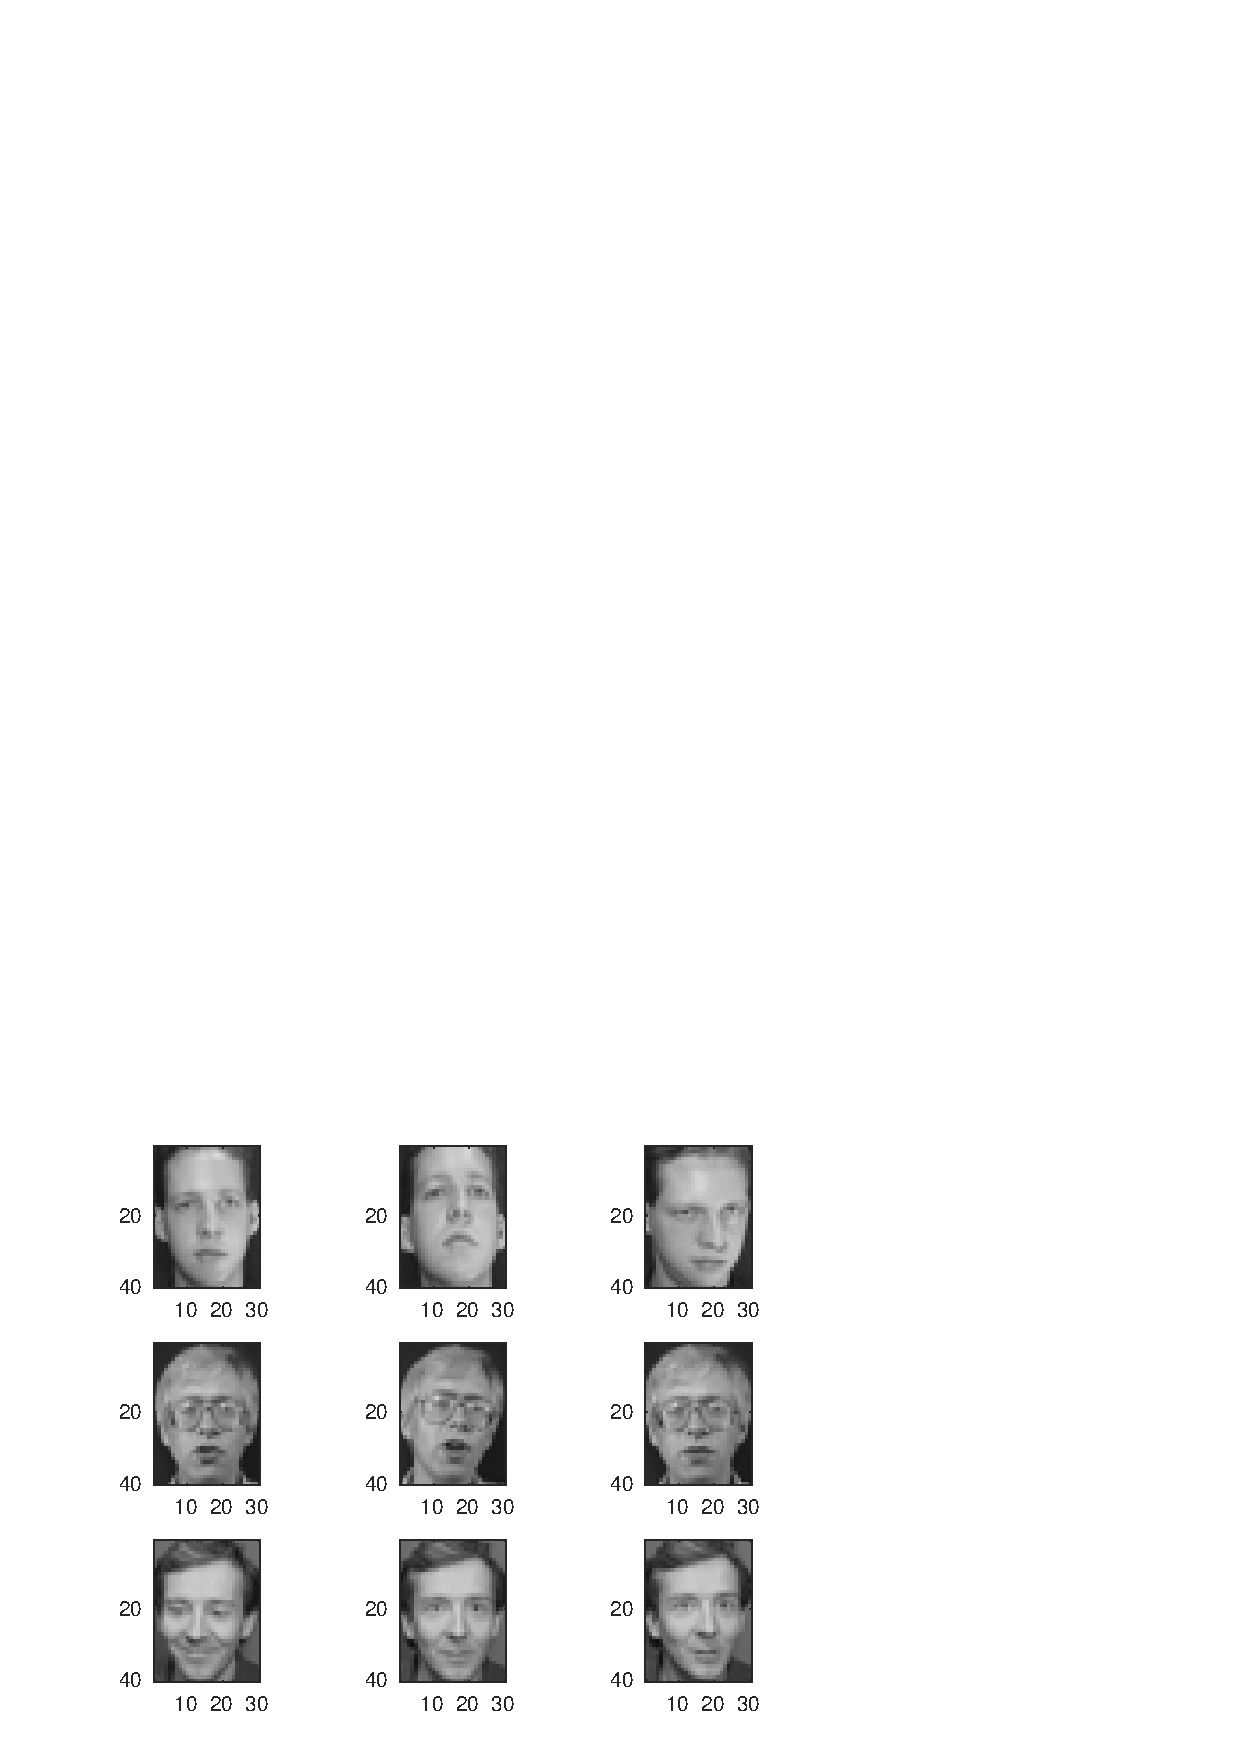
\includegraphics[width=0.4\textwidth]{fig/orl.jpg}
  \caption{ORL dataset sample}
\end{figure}

Each algorithm has been compared by execution time, and success rate (or accuracy). It can be seen that changing the hyperparameters of one can drastically improve its success rate, as the Nearest Sub-class Centroid Classifier shows for instance, with the given hyperparameters \{2,3,5\} corresponding to the number of sub-classes. The learning rate for the backpropagation algorithm has been set to 0.1, after experimentation and fine-tuning.
\\

INSERT MNIST SUCCESS RATE
\\

INSERT ORL SUCCESS RATE
\\

The bar diagrams showed in figure 3 and 4 clearly show that ...



%\input{src/conclusion.tex}
\begin{thebibliography}{00}
\bibitem{b1}  A. Iosifidis,  Machine Learning, Course Notes, Aarhus: Aarhus University, 2017
\bibitem{b2}  Y. LeCun, C. Cortes, C.J.C Burges. "The MNIST database of handwritten digits". Internet: http://yann.lecun.com/exdb/mnist/ [Dec. 6, 2017]. 
\bibitem{b3} AT\&T Laboratories Cambridge. "The ORL database of faces". Internet: https://www.cl.cam.ac.uk/research/dtg/attarchive/facedatabase.html, 2002. 

\end{thebibliography}




\end{document}
